\chapter{Формулы расчета излучения}\label{Formulae}

\section{Преобразование функции распределения фотонов}
Функция распределения фотонов задана в сферических координатах $n_{ph}(\epsilon,\mu,\phi)$. Рассмотрим переход в систему отсчета, движущуюся в направлении оси $z$ с лоренц-фактором $\gamma = 1/\sqrt{1-\beta^2}$. Количество частиц в элементе фазового пространства $N$ - инвариант.

\begin{equation}
	N = n_{ph}(\epsilon,\mu,\phi)d\epsilon d\mu d\phi dV = n'_{ph}(\epsilon',\mu',\phi')d\epsilon' d\mu' d\phi' dV'
\end{equation}

Для вычисления функции распределения движущейся системе отсчета необходимо вычислить якобиан матрицы перехода в движущуюся систему отсчета. С учеом того, что азимутальный угол $\phi' = \phi$ не изменяется при преобразованиях, и энергия и полярный угол не зависят от объема, занимаемого частицами, в общем виде матрица перехода выглядит как

\begin{equation}\label{generalJacobi}
J=\left(
\begin{array}{cccc}
\frac{d\epsilon'}{d\epsilon} & \frac{d\epsilon'}{d\mu}& 0 & 0\\
\frac{d\mu'}{d\epsilon} & \frac{d\mu'}{d\mu} & 0 & 0\\
0 & 0 & 1 & 0\\
\frac{dV'}{d\epsilon} & \frac{dV'}{d\mu} & 0 & \frac{dV'}{dV}
\end{array}
\right)
\end{equation}

Определитель такой матрицы можно разложить по последнему столбцу и получить, что

\begin{equation}
|J|=\frac{dV'}{dV}\left(\frac{d\epsilon'}{d\epsilon}\frac{d\mu'}{d\mu} - \frac{d\epsilon'}{d\mu}\frac{d\mu'}{d\epsilon}\right)
\end{equation}

Начнем с преобразования пространственного объема $V$. Один способ, используемый в п.10 т.2 Ландау-Лифшица \cite{LandauLifshitz2}, связан с переходом в собственную систему отсчета пучка движущихся частиц. Из этого можно получить, что объем преобразуется обратно энергии $dV'/dV= \epsilon/\epsilon'$. Этот результат правильный, но вывод не корректен для безмассовых частиц, у которых не существует собственной системы отсчета.

Поэтому мы вычислим изменение объема, содержащего рассматриваемые частицы. непосредственно из преобразований Лоренца. Рассмотрим поток частиц, равномерно распределенных вдоль оси $z$, с расстоянием $L$ между соседними частицами, и движущихся со одной скоростью $v$, направленной под углом $\theta$ к оси $z$ и введем величину $\mu = cos \theta$, как показано на рисунке \ref{VolumeTransform}.

\begin{figure}[h]
	\centering
	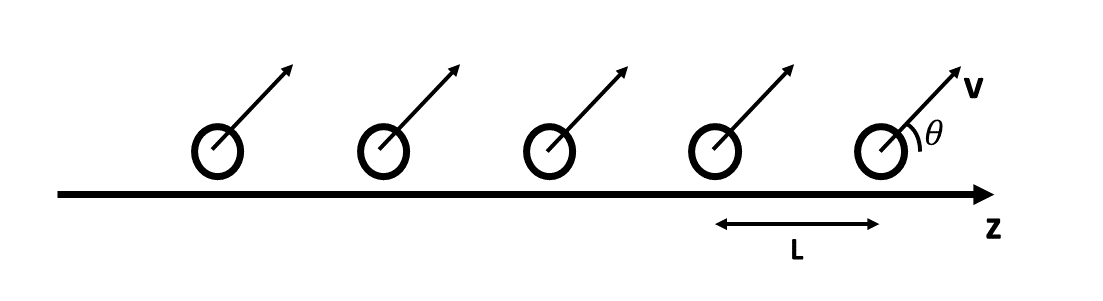
\includegraphics[width=12.5 cm]{./fig/VolumeTransform.png} 
	\caption{Пучок равномерно распределенных частиц, движущихся с одинаковыми скоростями}
	\label{VolumeTransform}
\end{figure}

В лабораторной системе i-тая частица в момент времени t имеет z-координату $z_i = i\cdot L + \mu v t$. Вычислим ее координаты в движущейся системе отсчета

\begin{equation}\label{lorentz_z}
\left(\begin{array}{c}
ct'\\
z'_i
\end{array}
\right)
= \left(
\begin{array}{cc}
\gamma & -\beta\gamma\\
-\beta\gamma & \gamma
\end{array}
\right)
\times
\left(\begin{array}{c}
ct\\
z_i
\end{array}
\right)
\end{equation}  

из этой системы можно получить, что значение координаты в движущейся системе равно $z'_i = \gamma z_i + (\gamma \mu v - c\beta \gamma)t$, но эти значения соответствуют одному моменту времени $t$ в лабораторной системе отсчета, в то время как для определения объема или концентрации в движущейся системе, нам нужны координаты частиц в один момент времени относительно движущейся системы. Поэтому выразим $t$ через $z_i$ и $t'$ и подставим в выражение для координат $z'_i$

\begin{equation}
t=\frac{t'+\gamma\beta z_i/c}{\gamma - \beta \mu v/c}
\end{equation}

и

\begin{equation}
z'_i=\gamma z_i +(\gamma \mu v - c\beta \gamma)\frac{t'+\gamma\beta z_i/c}{\gamma - \beta \mu v/c}=z_i\frac{1}{\gamma(1-\beta\mu v/c)} + t'\frac{\mu v/c - \beta}{1 - \beta \mu v/c}
\end{equation}

Второй член, содержащий $t'$ дает стандартную формулу для релятивистского сложения скоростей. А первый характеризует сокращение расстояний между частицами $L' = z'_{i+1}-z'_i = L/(\gamma(1-\beta\mu v/c))$. Расстояния вдоль поперечных направлений не изменяются, поэтому изменение объема будет таким же

\begin{equation} \label{volume}
V' = V/(\gamma(1-\beta\mu v/c))
\end{equation}

это тот же результат, что и приводимый Ландау и Лифшицем \cite{LandauLifshitz2}

Далее нужно найти выражения для $\epsilon'$ и $\mu'$, но их лучше рассмотреть в двух отдельных случаях - для безмассовых частиц и для массивных.

\subsection{Фотоны}

Рассмотрим преобразование вектора четырех-импульса для безмассовых частиц (фотонов), учитывая что оперечные компоненты не изменяются, а временная и продольная связаны как $p_z = \mu \epsilon$:

\begin{equation}\label{lorentz_ph}
	\left(\begin{array}{c}
		\epsilon'\\
		\mu'\epsilon'
	\end{array}
	\right)
	= \left(
	\begin{array}{cc}
		\gamma & -\beta\gamma\\
		-\beta\gamma & \gamma
	\end{array}
	\right)
	\times
	\left(\begin{array}{c}
		\epsilon\\
		\mu\epsilon
	\end{array}
	\right)
\end{equation}

Из первой строчки матрицы получаем уравнение для допплеровского сдвига энергии

\begin{equation}\label{doppler_ph}
	\epsilon'=\gamma(1-\mu\beta)\epsilon
\end{equation}

Вычислим производные новой энергии по старым координатам

\begin{equation}
	\frac{d\epsilon'}{d\epsilon}=\gamma(1-\mu\beta)
\end{equation}

\begin{equation}
	\frac{d\epsilon'}{d\mu}=-\gamma\beta\epsilon
\end{equation}

Из второй строчки матрицы получаем $\mu'\epsilon'=-\beta\gamma\epsilon+\gamma\mu\epsilon$.Подставив значение $\epsilon'$ из \ref{doppler_ph} и сократив $\epsilon$ получим уравнение аберрации света

\begin{equation}\label{aberration_ph}
	\mu'=\frac{\mu-\beta}{1-\mu\beta}
\end{equation}

Заметим, что угол наклона луча в новой системе не зависит от энергии в старой системе. Вычислим частноую производную $\frac{d\mu'}{d\mu}$

\begin{equation}
	\frac{d\mu'}{d\mu}=\frac{d}{d\mu}\frac{1}{\beta}\frac{\beta\mu-1+1-\beta^2}{1-\mu\beta}=\frac{d}{d\mu}\frac{1}{\beta}\frac{1-\beta^2}{1-\mu\beta}=\frac{1-\beta^2}{(1-\mu\beta)^2}=\frac{1}{\gamma^2(1-\mu\beta)^2}
\end{equation}

Матрица якоби преобразования координат выглядит следующим образом

\begin{equation}
	J=\left(
	\begin{array}{cccc}
		\frac{d\epsilon'}{d\epsilon} & \frac{d\epsilon'}{d\mu}& 0 & 0\\
		0 & \frac{d\mu'}{d\mu} & 0 & 0\\
		0 & 0 & 1 & 0\\
		0 & \frac{dV'}{d\mu} & 0 & \frac{dV'}{dV}
	\end{array}
	\right)
\end{equation}

При такой матрице якобиан, к счастью, равен произведению диагональных членов

\begin{equation}\label{jacobian_ph}
	\frac{D(\epsilon',\mu',\phi',V')}{D(\epsilon,\mu,\phi,V)}=\frac{d\epsilon'}{d\epsilon}\frac{d\mu'}{d\mu}\frac{dV'}{dV}=\gamma(1-\mu\beta)\frac{1}{\gamma^2(1-\mu\beta)^2}\frac{1}{\gamma(1-\mu\beta)}=\frac{1}{\gamma^2(1-\mu\beta)^2}
\end{equation}

И в итоге функция распределения фотонов преобразуется с помощью деления на вычисленный якобиан

\begin{equation}\label{distribution_ph}
	n'_{ph}(\epsilon',\mu',\phi') = \frac{n_{ph}(\epsilon,\mu,\phi)}{\frac{D(\epsilon',\mu',\phi',V')}{D(\epsilon,\mu,\phi,V)}}=\gamma^2(1-\mu\beta)^2 n_{ph}(\epsilon,\mu,\phi)
\end{equation}

\subsection{Массивные частицы}

Для массивных частиц выражения для $\epsilon'$ и $\mu'$ намного сложнее. В этом случае $p_z = \mu \sqrt{\epsilon^2 - m^2 c^4}/c$ где $m$ масса частиц, и преобразования Лоренца выглядят следующим образом

\begin{equation}\label{lorentz_m}
\left(\begin{array}{c}
\epsilon'\\
\mu'\sqrt{{\epsilon'}^2 - m^2 c^4}
\end{array}
\right)
= \left(
\begin{array}{cc}
\gamma & -\beta\gamma\\
-\beta\gamma & \gamma
\end{array}
\right)
\times
\left(\begin{array}{c}
\epsilon\\
\mu\sqrt{{\epsilon}^2-m^2 c^4}
\end{array}
\right)
\end{equation}

и выражения для $\epsilon'$ и $\mu'$

\begin{equation}
\epsilon' = \gamma\epsilon-\beta\gamma\mu\sqrt{\epsilon^2-m^2 c^4}
\end{equation}

\begin{equation}
\mu' = \frac{-\beta\gamma\epsilon+\gamma\mu\sqrt{{\epsilon}^2-m^2 c^4}}{\sqrt{{\epsilon^2 - m^2 c^4}}}
\end{equation}

Выражения для преобразования объемав переменных $\epsilon$ и $\mu$

\begin{equation}
V'=\frac{V}{\gamma(1-\mu\beta\sqrt{{\epsilon}^2-m^2 c^4}/\epsilon)}
\end{equation}

Выражения для частных производных $\epsilon'$, $\mu'$, $V'$ и особенно для якобиана выглядят устрашающе, поэтому здесь мы приведем только финальный результат преобразования функции распределения в единицах $c = 1$

\begin{equation}
\frac{n'_{m}(\epsilon',\mu',\phi')}{n_{m}(\epsilon,\mu,\phi)}= \frac{\gamma(\epsilon-\mu\sqrt{{\epsilon}^2-m^2}\beta)(\gamma^2\epsilon^2-m^2 + \mu^2 ((\epsilon^2-m^2)(\gamma^2-1)) - 2\mu\epsilon\gamma^2\beta\sqrt{\epsilon^2-m^2})^{3/2}}{\epsilon(((\gamma^2-1)(\epsilon^2-m^2)\mu^2 + \gamma^2\epsilon^2 - m^2)\sqrt{\epsilon^2-m^2}-2\mu\epsilon\gamma(\epsilon^2 - m^2)\sqrt{\gamma^2 - 1})}
\end{equation}

\section{Комптоновское рассеяние}
Рассмотрим рассеяние фотонов на одном электроне, движущемся вдоль ось z, см \cite{Dubus}. Сечение Клейна-Нишины в системе покоя электрона равно

\begin{equation}\label{KleinNishina}
\frac{d\sigma}{d\epsilon_1'd\Omega_1'}=\frac{{r_e}^2}{2}\left(\frac{\epsilon_1'}{\epsilon_0'}\right)^2\left(\frac{\epsilon_1'}{\epsilon_0'}+\frac{\epsilon_0'}{\epsilon_1'}-\sin^2\Theta'\right) \delta\left(\epsilon_1' - \frac{\epsilon_0'}{1+\frac{\epsilon_0'}{m_e c^2}(1 - \cos \Theta')}\right)
\end{equation}

Где $r_e$ - классический радиус электрона, $\epsilon_0'$ и $\epsilon_1'$ - энергии начального и конечного фотона, соответственно, $\Theta'$ - угол между начальным и конечным фотоном, определяемый выражением $\cos\Theta' =\cos \theta_0' \cos \theta_1' + \sin \theta_0' \sin \theta_1' \cos(\phi_1' - \phi_0')$. Штрихованные индексы относятся к системе отсчета электрона. При этом начальная и конечная энергии фотонов оказываются связаны соотношениями

\begin{equation}
	\epsilon_1'=\frac{\epsilon_0'}{1+\frac{\epsilon_0'}{m_e c^2}(1 - \cos \Theta')}	
\end{equation}

\begin{equation}
	\epsilon_0'=\frac{\epsilon_1'}{1-\frac{\epsilon_1'}{m_e c^2}(1 - \cos \Theta')}
\end{equation}

Число фотонов, рассеявшихся в заданный телесный угол в единицу времени в промежуток энергии в системе покоя электрона равно

\begin{equation}
\frac{dN'}{dt'd\epsilon_1'd\Omega_1'}=\int c \frac{d\sigma}{d\epsilon_1'd\Omega_1'} \frac{dn'}{d\epsilon_0'd\Omega_0'}d\Omega_0'd\epsilon'_0
\end{equation}

Перепишем дельта-функцию через энергию начального фотона с помощью соотношения 

\begin{equation}
	\delta(f(x)) = \sum \frac{\delta(x-x_k)}{|f'(x_k)|}
\end{equation}

где $x_k$ - корни функции $f(x)$. Производная выражения внутри дельта-функции равна

\begin{equation}
	\frac{d\epsilon_1'}{d\epsilon_0'}=\frac{1}{(1+\frac{\epsilon_0'}{m_e c^2}(1 - \cos \Theta'))^2}
\end{equation}

и она сократится с квадратом отношения энергий в формуле для сечения. Функцию распределения начальных фотонов выразим в лабораторной системе с помощью выражения \ref{distribution_ph}.

\begin{equation}
\frac{dN'}{dt'd\epsilon_1'd\Omega_1'}=\int \frac{r_e^2 c}{2} \gamma_e^2 (1 - \mu_0 \beta_e)^2 \left(\frac{\epsilon_1'}{\epsilon_0'}+\frac{\epsilon_0'}{\epsilon_1'}-\sin^2\Theta'\right)\frac{dn}{d\epsilon_0 d\Omega_0} \delta\left(\epsilon_0' - \frac{\epsilon_1'}{1-\frac{\epsilon_1'}{m_e c^2}(1 - \cos \Theta')}\right) d\epsilon_0'd\mu_0' d\phi_0'
\end{equation}

Теперь избавимся от дельта-функции, проинтегрировав по $\epsilon'_0$.

\begin{equation}
\frac{dN'}{dt'd\epsilon_1'd\Omega_1'}=\int \frac{r_e^2 c}{2} \gamma_e^2 (1 - \mu_0 \beta_e)^2 \left(1 + \cos^2\Theta'+\left(\frac{\epsilon_1'}{m_e c^2}\right)^2\frac{(1-\cos\Theta')^2}{1-\frac{\epsilon_1'}{m_e c^2}(1 - \cos \Theta')}\right)\frac{dn}{d\epsilon_0 d\Omega_0}d\mu_0' d\phi_0'
\end{equation}

Осталось перевести количество рассеяных фотонов в лабораторную систему отсчета $\frac{dN}{dt d\epsilon_1 d\Omega_1} = \frac{dN'}{dt' d\epsilon_1' d\Omega_1'}\frac{dt'}{dt}\frac{d\epsilon_1'}{d\epsilon_1}\frac{d\Omega_1'}{d\Omega_1}$. Используя то, что $dt = \gamma_e dt'$, $\epsilon = \frac{1}{\gamma_e(1 -\mu_1\beta_e)}\epsilon'$ и $\mu_1' = \frac{\mu_1-\beta_e}{1-\mu_1 \beta_e}$ получим

\begin{equation} \label{compton_elframe}
\frac{dN}{dt d\epsilon_1 d\Omega_1}=\int \frac{r_e^2 c}{2} \frac{(1 - \mu_0 \beta_e)^2}{1-\mu_1\beta_e} \left(1 + \cos^2\Theta'+\left(\frac{\epsilon_1'}{m_e c^2}\right)^2\frac{(1-\cos\Theta')^2}{1-\frac{\epsilon_1'}{m_e c^2}(1 - \cos \Theta')}\right)\frac{dn}{d\epsilon_0 d\Omega_0}d\mu_0' d\phi_0'	
\end{equation}

Так же может быть удобно интегрировать в переменных лабораторной системы расчета, тогда выражение для потока фотонов будет следующим

\begin{equation}\label{compton_labframe}
\frac{dN}{dt d\epsilon_1 d\Omega_1}=\int \frac{r_e^2 c}{2} \frac{1}{\gamma_e^2(1-\mu_1\beta_e)} \left(1 + \cos^2\Theta'+\left(\frac{\epsilon_1'}{m_e c^2}\right)^2\frac{(1-\cos\Theta')^2}{1-\frac{\epsilon_1'}{m_e c^2}(1 - \cos \Theta')}\right)\frac{dn}{d\epsilon_0 d\Omega_0}d\mu_0 d\phi_0
\end{equation}

При интегрировании нужно выразить углы в лабораторной системе отсчета $\mu_0, \phi_0$ через переменные интегрирования $\mu_0', \phi_0'$. Для расчета рассеяния на распределении электронов нужно проинтегрировать формулу \ref{compton_elframe} или \ref{compton_labframe} с функцией распределения электронов, нормированной на концентрацию частиц частиц. При этом надо учесть разные направления движения электронов и произвести повороты углов.

В коде реализовано вычисления потоков в терминах энергетической плотности потока энергии в единицах $\textbf{см}^{-2}\textbf{с}^{-1}$. Для вычисления этой величины нужно домножить число рассеянных фотонов на энергию, поделить на квадрат расстояния до источника и проинтегрировать по объему источника.

\begin{equation}\label{comtonKlein}
F(\epsilon_1)=\frac{\epsilon_1}{D^2}\int \frac{dN}{dt d\epsilon_1 d\Omega_1} \frac{dn_e}{d\epsilon_e d\Omega_e} dV d\epsilon_e d\Omega_e
\end{equation}

При рассмотрении процессов, связанных с электронами высоких энергий $\gamma_e \approx 10^8$ относительные численные погрешности вычислений могут быть очень велики, так как $\beta_e$ и $\mu_0, \mu_1, \cos \Theta'$ оказываются слишком близки к единице и стандартный тип double может не разрешать это отличие. Поэтому для численных вычислений оказывается полезным ввести следующие вспомогательные величины:

\begin{equation}
	\delta_e = 1 - \beta_e
\end{equation}

\begin{equation}
	\text{versin}~\theta = 1 - \cos \theta
\end{equation}

Тогда выражения вида $1 - \mu \beta_e$ в этих величинах перепишется как

\begin{equation}
	1 - \mu \beta_e =\text{versin}~\theta + \delta_e - \text{versin}~\theta~\delta_e
\end{equation}

а выражение для угла между конечным и начальным фотоном как

\begin{equation}
	1 - \cos \Theta' = \text{versin}~\theta_0' + \text{versin}~\theta_1' - \text{versin}~ \theta_0' \text{versin}~\theta_1' - \sin \theta_0'\sin \theta_1' \cos(\phi_1'-\phi_0')
\end{equation}

С использованием данных выражений значительно повышается точность и максимальные доступные к рассмотрению энергии фотонов и электронов.

В случае изотропных функций распределения фотонов и релятивистских электронов можно произвести аналитическое интегрирование по угловым переменным \cite{JonesCompton, BykovUvarov2000}, и тогда для вычисления излучения достаточно лишь провести интегрирования по энергиям по формуле

\begin{equation}
F(\epsilon_1)=\frac{\epsilon_1}{D^2}\int \frac{2 \pi r_e^2 \beta_e c}{\epsilon_0 \gamma_e^2} \frac{dn_{ph}}{d\epsilon_0}\frac{dn_e}{d\epsilon_e}(2 q~ \ln(q)+1+q-2q^2+\frac{q^2(1-q)\Gamma^2}{2(1+q\Gamma)})d\epsilon_0 d\epsilon_e dV
\end{equation}

где $\Gamma=4\epsilon_0\gamma_e/m_e c^2$, $q=\epsilon_1/((\gamma_e m_e c^2-\epsilon_1)\Gamma)$.

\section{Синхротронное излучение}
Процесс синхротронного излучения хороши известен и описан в классических работах, например \cite{Ginzburg1975}. Но так же возможен и процесс синхротронного поглощения. Сечение этого процесса описано в работе Гизеллини и Свенсона \cite{Ghisellini1991}. В коде вычисляются спектральная плотность мощности излучения единицы объема и линейный коэффициент поглощения, описанные в работе \cite{Ghisellini}. Спектральная плотность мощности излучения единицы объема вещества определеяется формулой

\begin{equation} \label{emission}
	I(\nu)=\int_{E_{min}}^{E_{max}} dE \frac {\sqrt {3}{e}^{3}n F(E) B \sin ( \phi)}{{m_e}{c}^{2}}
	\frac{\nu}{\nu_c}\int_{\frac {\nu}{\nu_c}}^{\infty }\it K_{5/3}(x)dx,
\end{equation}

где $\phi$ это угол межде вектором магнитного поля и лучом зрения, $\displaystyle\nu_{c}$ критическая частота, определяемая выражением $\displaystyle\nu_{c} = 3 e^{2} B \sin(\phi) E^{2}/4\pi {m_{e}}^{3} c^{5}$, и~$K_{5/3}$ - функция МакДональда.
Коэффициент поглощения для фотонов, распростроняющихся вдоль луча зрения равен

\begin{equation}\label{absorption}
	k(\nu)=\int_{E_{min}}^{E_{max}}dE\frac {\sqrt {3}{e}^{3}}{8\pi m_e \nu^2}\frac{n B\sin(\phi)}{E^2}
	\frac{d}{dE} E^2 F(E)\frac {\nu}{ \nu_c}\int_{\frac {\nu}{ \nu_c}}^{\infty }K_{5/3}(x) dx.
\end{equation}

\section{Распад пионов}

\section{Тормозное излучение}